
% Set document class and font size
\documentclass[letterpaper, 11pt]{article}
\usepackage[utf8]{inputenc}

% Package imports
\usepackage{setspace, longtable, graphicx, hyphenat, hyperref, fancyhdr, ifthen, everypage, enumitem, amsmath, setspace}
\usepackage{array}
\usepackage{tabularx}


\makeatletter
\newcommand*\bigcdot{\mathpalette\bigcdot@{1.0}}
\newcommand*\bigcdot@[2]{\mathbin{\vcenter{\hbox{\scalebox{#2}{$\m@th#1\bullet$}}}}}
\makeatother

\usepackage[backend=biber]{biblatex}
\addbibresource{sample.bib}



% --- Page layout settings ---

% Set page margins
\usepackage[left=1.5cm, right=1.5cm, bottom=1.0cm, top=1.0cm]{geometry}

% --- Page formatting ---

% Set link colors
\usepackage[dvipsnames]{xcolor}
\urlstyle{sf}
\hypersetup{colorlinks=true, linkcolor=Blue, urlcolor=Blue}

% Set font to Libertine, including math support
\usepackage{libertine}
\usepackage[libertine]{newtxmath}

% Remove page numbering
\pagenumbering{gobble}

% --- Document starts here ---

\begin{document}


% set no indent
\setlength\parindent{0pt}\textbf{}

\hfill%
\begin{minipage}{0.79\textwidth}\flushleft
\huge{\bf{Eliott Johnson}}\\
\normalsize
Sep 12, 1993 $\bigcdot$ Swiss nationality $\bigcdot$  Linkedin: \href{https://www.linkedin.com/in/eliottjohnson/}{eliottjohnson}\\Github:  \href{https://github.com/eliottjohnson}{github.com/eliottjohnson}
\end{minipage}
\begin{minipage}{0.19\textwidth}% adapt widths of minipages to your needs
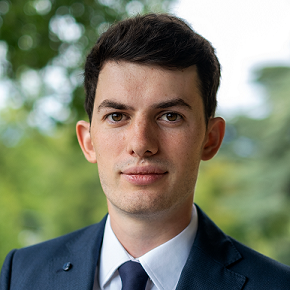
\includegraphics[width=\linewidth]{LinkedInProfilPic.png}
\end{minipage}%
\vspace{0.25cm}

\noindent\rule{\textwidth}{1pt}

% --- Section: Education ---
\begin{center}
\large\bf{EDUCATION}
\end{center}

\begin{tabularx}{1.0\textwidth} { 
   >{\raggedright\arraybackslash\hsize=1.5\hsize\linewidth=\hsize}X 
   >{\raggedleft\arraybackslash\hsize=.5\hsize\linewidth=\hsize}X }
\normalsize
\bf{University of Geneva} & Geneva, CH \\
\normalfont M.Sc.\ in Particles Physics & Sep 2018 -- Jun 2020  \\  
Quantum Electrodynamics \& Chromodynamics, Quantum Field Theory, General Relativity, Cosmic Ray Physics, Detectors and Accelerators &
\end{tabularx}
\vspace{0.25cm}



\begin{tabularx}{1.0\textwidth} { 
   >{\raggedright\arraybackslash\hsize=1.5\hsize\linewidth=\hsize}X 
   >{\raggedleft\arraybackslash\hsize=.5\hsize\linewidth=\hsize}X }
\normalsize
\bf{University of Geneva} & Geneva, CH \\
\normalfont B.Sc.\ in Physics & Sep 2015 -- Jun 2018  \\  
Classical Mechanics, Electrodynamics, Linear Algebra, Complex \& Fourier Analysis, Astrophysics, Statistical Mechanics and Solid State Physics &
\end{tabularx}
\vspace{0.25cm}

\begin{tabularx}{1.0\textwidth} { 
   >{\raggedright\arraybackslash\hsize=1.5\hsize\linewidth=\hsize}X 
   >{\raggedleft\arraybackslash\hsize=.5\hsize\linewidth=\hsize}X }
\normalsize
\bf{Swiss Federal Institute of Technology Lausanne (EPFL)} & Lausanne, CH \\
\normalfont Mechanical engineering & Sep 2014 -- Jun 2015\\
Analysis, Linear Algebra, Classical Mechanics, Thermodynamics, Mechanical construction, Global issues, Communication, Structural mechanics, Materials, Electricity
\end{tabularx}
\vspace{0.25cm}

\begin{tabularx}{1.0\textwidth} { 
   >{\raggedright\arraybackslash\hsize=1.5\hsize\linewidth=\hsize}X 
   >{\raggedleft\arraybackslash\hsize=.5\hsize\linewidth=\hsize}X }
\normalsize
\bf{Swiss Federal Institute of Technology Zürich (ETH)} & Zürich, CH \\
\normalfont Mechanical engineering & Sep 2013 -- Jun 2014 \\
Analysis, Linear Algebra, Classical mechanics, Materials and manufacturing, Technical drawing \& CAD, Chemistry, Machine elements, Computer science, Innovation process \& project
\end{tabularx}
\vspace{0.25cm}

% --- Section: Work Experience ---
\begin{center}
\noindent\rule{0.75\textwidth}{1pt}
\end{center}

\begin{center}
\large\bf{WORK EXPERIENCE}
\end{center}

\begin{tabularx}{1.0\textwidth} { 
   >{\raggedright\arraybackslash\hsize=1.5\hsize\linewidth=\hsize}X 
   >{\raggedleft\arraybackslash\hsize=.5\hsize\linewidth=\hsize}X }
\normalsize
\bf{Junior Fellowship - European Organization for Nuclear Research (CERN)} & Geneva, CH\\
\normalfont \begin{itemize}[leftmargin=*,noitemsep,topsep=0pt]
\item Accelerator physicist responsible for the conception, studies, design and commissioning of beam transfer lines and injection/extraction systems
\item Checking and improving the performance of existing injection/extraction systems and beam lines and responsible for scheduling, resources planning and coordination of work packages from beamline design to beam commissioning
\end{itemize} & Jun 2021 -- Present
\end{tabularx}

\begin{tabularx}{1.0\textwidth} { 
   >{\raggedright\arraybackslash\hsize=1.5\hsize\linewidth=\hsize}X 
   >{\raggedleft\arraybackslash\hsize=.5\hsize\linewidth=\hsize}X }
\normalsize
\bf{Airline Customer Service Agent - Swissport} & Geneva, CH\\
\normalfont \begin{itemize}[leftmargin=*,noitemsep,topsep=0pt]
\item Managed passenger logistics between terminal and aircraft, ensuring efficient processing of travel documents and boarding passes.
\item Obtained international airport tarmac security clearance, demonstrating a high level of trust and responsibility.
\item Adapted to a flexible schedule, including evenings, nights, weekends, and holidays, to maintain high-quality customer service.
\end{itemize} & Nov 2018 -- Jun 2021
\end{tabularx}

\begin{tabularx}{1.0\textwidth} { 
   >{\raggedright\arraybackslash\hsize=1.5\hsize\linewidth=\hsize}X 
   >{\raggedleft\arraybackslash\hsize=.5\hsize\linewidth=\hsize}X }
\normalsize
\bf{European Organization for Nuclear Research (CERN)} & Geneva, CH\\
\normalfont \begin{itemize}[leftmargin=*,noitemsep,topsep=0pt]
\item Contributed to the development of FASER, focusing on the detection of weakly interacting massive particles, and enhancing experimental reach.
\item Led quality assurance and development of the signal triggering system, integrating my designs into the workflow of an international scientific team of over 30 members.
\end{itemize} & Sep 2019 -- Jul 2020
\end{tabularx}

\begin{tabularx}{1.0\textwidth} { 
   >{\raggedright\arraybackslash\hsize=1.5\hsize\linewidth=\hsize}X 
   >{\raggedleft\arraybackslash\hsize=.5\hsize\linewidth=\hsize}X }
\normalsize
\bf{Physics Laboratory Assistant - University of Geneva \& ECG Jean-Piaget} & Geneva, CH\\
\normalfont \begin{itemize}[leftmargin=*,noitemsep,topsep=0pt]
\item Mentored and guided high school and university students in hands-on experiments, fostering practical skills and scientific inquiry.
\end{itemize} & Sep 2018 -- Aug 2020
\end{tabularx}

\begin{tabularx}{1.0\textwidth} { 
   >{\raggedright\arraybackslash\hsize=1.5\hsize\linewidth=\hsize}X 
   >{\raggedleft\arraybackslash\hsize=.5\hsize\linewidth=\hsize}X }
\normalsize
\bf{Mechanical Engineering Internship - Rolex} & Geneva, CH\\
\normalfont \begin{itemize}[leftmargin=*,noitemsep,topsep=0pt]
\item Gained comprehensive insight into the stages of high-quality watch production, from gold melting to ceramic milling, contributing to the creation of luxury watches.
\end{itemize} & Jan 2014 --  Feb 2014
\end{tabularx}


% --- Section: Additional Experience ---
\begin{center}
\noindent\rule{0.75\textwidth}{1pt}
\end{center}

\begin{center}
\large\bf{ADDITIONAL EXPERIENCE}
\end{center}

\begin{tabularx}{1.0\textwidth} { 
   >{\raggedright\arraybackslash\hsize=1.5\hsize\linewidth=\hsize}X 
   >{\raggedleft\arraybackslash\hsize=.5\hsize\linewidth=\hsize}X }
\normalsize
\bf{CERN accelerator School (CAS)} & Geneva, CH \\
\normalfont Training courses on accelerator physics and associated technologies at different levels for physicists, engineers, technicians and students & Jul 2018
\end{tabularx}
\vspace{0.25cm}

\begin{tabularx}{1.0\textwidth} { 
   >{\raggedright\arraybackslash\hsize=1.5\hsize\linewidth=\hsize}X 
   >{\raggedleft\arraybackslash\hsize=.5\hsize\linewidth=\hsize}X }
\normalsize
\bf{University of Goettingen} & Goettingen, GER \\
\normalfont Hadron collider physics school (HASCO) & Jul 2018 \\
\end{tabularx}
\vspace{0.25cm}

\begin{tabularx}{1.0\textwidth} { 
   >{\raggedright\arraybackslash\hsize=1.5\hsize\linewidth=\hsize}X 
   >{\raggedleft\arraybackslash\hsize=.5\hsize\linewidth=\hsize}X }
\normalsize
\bf{Expert in Radioprotection - CHUV} & Lausanne, CH\\
\normalfont 
Qualified as a radiation protection expert in the use of unsealed radioactive materials in a B/C work area & Feb -- Jul 2019
\end{tabularx}
\vspace{0.25cm}

\begin{tabularx}{1.0\textwidth} { 
   >{\raggedright\arraybackslash\hsize=1.5\hsize\linewidth=\hsize}X 
   >{\raggedleft\arraybackslash\hsize=.5\hsize\linewidth=\hsize}X }
\normalsize
\bf{Aviation} & CH\\
\normalfont \begin{itemize}[leftmargin=*,noitemsep,topsep=0pt]
\item PPL, Medical Class 2, SEP (Land), English Level 6, Aerobatics (A), Night (A)
\item Participated three times in the Swiss national aerobatics championship
\item Aviation soldier in the Swiss military on the F-5 Tiger and F-18 Hornet
\item Recommended by SPHAIR to become a military and/or a commercial pilot
\end{itemize} & 2014 - Present
\end{tabularx}


% --- Section: Skills ---
\begin{center}
\noindent\rule{0.75\textwidth}{1pt}
\end{center}

\begin{center}
\large\bf{SKILLS}
\end{center}

\begin{tabularx}{1.0\textwidth} { 
   >{\raggedright\arraybackslash\hsize=1.5\hsize\linewidth=\hsize}X 
   >{\raggedleft\arraybackslash\hsize=.5\hsize\linewidth=\hsize}X }
\normalsize
\bf{Languages} & \\
\normalfont
French - Native & \\
English - Full professional & \\
German - Intermediate 
\end{tabularx}
\vspace{0.25cm}

\begin{tabularx}{1.0\textwidth} { 
   >{\raggedright\arraybackslash\hsize=1.5\hsize\linewidth=\hsize}X 
   >{\raggedleft\arraybackslash\hsize=.5\hsize\linewidth=\hsize}X }
\normalsize
\bf{Computer Skills} & \\
\normalfont \begin{itemize}[leftmargin=*,noitemsep,topsep=0pt]
\item \textbf{Microsoft Office Suite:}  Excel, Word, PowerPoint, Outlook
\item \textbf{Programming:} Python, C++, Git, MAD-X, XSuite, HTML, CSS
\item \textbf{Data Analysis:} Matplotlib, Pandas, NumPy, SciPy, Seaborn, Scikit-learn, Jupyter Notebook, Apache Spark, SQL, Mathematica, Matlab, Root, Igor
\item \textbf{Other:} Linux, LateX, CAD, Arduino, 3D printing, Adobe Premiere, Computer building
\end{itemize} & 
\end{tabularx}

\newpage
% --- Section: Publication ---
\begin{center}
\noindent\rule{0.75\textwidth}{1pt}
\end{center}

\begin{center}
\large\bf{PUBLICATION}
\end{center}

\nocite{*}

\printbibliography[keyword=primaryauthor, title=\normalsize Primary Author, heading=subbibliography]
\printbibliography[keyword=secondaryauthor, title=\normalsize Co-Author, heading=subbibliography]


% --- End of CV! ---


\end{document}
